\documentclass{beamer}
\usepackage{moreverb} 
\usepackage{listings}
\usepackage{mflogo}
% imprimir
% \documentclass[handout]{beamer} 
% \usepackage{pgfpages}
% \pgfpagesuselayout{4 on 1}[a4paper,landscape,border shrink=5mm]

\mode<presentation> {
  \usetheme{Warsaw}
  \setbeamercovered{transparent}
}

\usebackgroundtemplate{
\includegraphics[width=\paperwidth]{format/libresoft-bg.png}}
% \usepackage[spanish]{babel}
\usepackage[utf8]{inputenc}
\usepackage{graphics}
\usepackage{amssymb} % Simbolos matematicos

%% Metadatos del PDF.
\hypersetup{  
  pdftitle={LaTeX in a Nutshell},
  pdfauthor={Miguel Vidal},
  pdfcreator={GSyC/Libresoft},
  pdfproducer=PDFLaTeX,
  pdfsubject={Master on Free Software},
}
%%

\defbeamertemplate*{footline}{shadow theme}
{%
  \leavevmode%
  \hbox{\begin{beamercolorbox}[wd=.5\paperwidth,ht=2.5ex,dp=1.125ex,leftskip=.3cm plus1fil,rightskip=.3cm]{author in head/foot}%
    \usebeamerfont{author in head/foot}\insertframenumber\,/\,\inserttotalframenumber\hfill
\includegraphics[scale=0.40]{format/cc-by-80x15.png} \hspace{0.1cm}\insertshortauthor 
% \usebeamerfont{author in head/foot} 
\includegraphics[width=0.7cm]{format/cc-by.png} \hfill\insertshortauthor
  \end{beamercolorbox}%
  \begin{beamercolorbox}[wd=.5\paperwidth,ht=2.5ex,dp=1.125ex,leftskip=.3cm,rightskip=.3cm plus1fil]{title in head/foot}%
    \usebeamerfont{title in head/foot}\insertshorttitle%
  \end{beamercolorbox}}%
  \vskip0pt%
}

\begin{document}

\title{\LaTeX{} in a Nutshell}
\subtitle{Master on Libre Software 2011-12}
\institute{\texttt{http://gsyc.urjc.es/\~{}mvidal} \\ Twitter: \texttt{@mvidallopez}}
\author{Miguel Vidal} 
%\date{\today}
\date{September 22, 2011}

\frame{
\maketitle
\begin{center}

\includegraphics[width=6cm]{format/gsyc-urjc}
\end{center}
}

%% License slide
\begin{frame}
  \vspace{2cm}
  \begin{center}
    {\small (cc) 2011 Miguel Vidal, LibreSoft} \\
%    \vspace{0.25cm}
    \medskip
    {\scriptsize This work is licensed under \\ a Creative Commons Attribution 3.0 License}
%    \vspace{0.10cm}
  \end{center}
  \begin{center}
    \href{http://creativecommons.org/licenses/by/3.0/es}{
\includegraphics[width=2cm]{format/cc-by.png}} \\
    {\tiny \url{http://creativecommons.org/licenses/by/3.0}}
  \end{center}
\end{frame}%%

\usebackgroundtemplate{}

\AtBeginSubsection[]
{
  \begin{frame}<beamer>{Table of Contents}
    \tableofcontents[currentsection,currentsubsection]
  \end{frame}
}

%%%%%%%%%%%%%%%%%%%%%%%%%%%%%%%%%%%%%%%%%%%%%%%%%%%%%%%%%%%%%%%%%%%%%%%
\section{What is (La)\TeX}
%%%%%%%%%%%%%%%%%%%%%%%%%%%%%%%%%%%%%%%%%%%%%%%%%%%%%%%%%%%%%%%%%%%%%%%

\subsection{\TeX}
\begin{frame}
\frametitle{What is \TeX}

\begin{itemize}
\item A computer program (\textit{language} and \textit{interpreter}) created by Donald Knuth in 1977.
\item Knuth wrote the \TeX{} typesetting engine to explore potential of the digital printing equipment.
\item He aimed to revert trend of deteriorating typographical quality that affected his own books and articles.
\item Two main aims: highest \alert{quality} and highest \alert{durability}.
\end{itemize}

\end{frame}

%%%%%%%%%%%%%%%%%%%%%%%%%%%%%%%%%%%%%%%%%%%%%%%%%%%%%%%%%%%%%%%%%%%%%%%

\begin{frame}
\frametitle{What is \TeX}

\begin{itemize}
\item \TeX{} as we use it today was released in 1982, with some slight enhancements added
in 1989 (8-bit characters support).
\item One of the most sophisticated digital typographical systems (``The greatest contribution in the printing world since Gutenberg''). 
\item Popular in academia, especially in mathematics, computer science, engineering, and physics. 
\item Free software (``public domain'' dedication): but any modified version must not be called \TeX!
\end{itemize}

\end{frame}




%%%%%%%%%%%%%%%%%%%%%%%%%%%%%%%%%%%%%%%%%%%%%%%%%%%%%%%%%%%%%%%%%%%%%%%

\begin{frame}
\frametitle{What is \TeX}

\begin{itemize}
\item \TeX{} understands about 300 low-level commands (``primitives''). Primitives are rarely used directly by users.
\item The smallest unit of length handled by TeX is 0,000005356mm! (\textit{scaled point}, 1 mm = 186712sp) 
\item Functionality is provided by \alert{format files} (predumped memory images of \TeX{} after large macro collections have been loaded).
\end{itemize}

\end{frame}

%%%%%%%%%%%%%%%%%%%%%%%%%%%%%%%%%%%%%%%%%%%%%%%%%%%%%%%%%%%%%%%%%%%%%%%

\begin{frame}
\frametitle{What is \TeX}

\begin{itemize}
\item Written in a `literate' programming language called Web.
\item TRIP and TRAP tests (``conformance test''): portable, same output with all versions. 
\item The design was frozen (and dedicated to Public Domain) in October 1990 (v3.1* --$\pi$--, no new features, only bug fixes).
\end{itemize}

\end{frame}



%%%%%%%%%%%%%%%%%%%%%%%%%%%%%%%%%%%%%%%%%%%%%%%%%%%%%%%%%%%%%%%%%%%%%%%

\begin{frame}[fragile] 
\frametitle{\MF}

\begin{itemize}
\item Font description language to describe characters (glyphs) algorithmically with geometrical equations.
\item It uses Bézier curves (vector graphics). 
\item Also created by Knuth but not strictly part of \TeX.
\item It is possible to use \TeX{} and \LaTeX{} without \MF. Adobe PostScript fonts may be used instead.
\end{itemize}

\end{frame}

%%%%%%%%%%%%%%%%%%%%%%%%%%%%%%%%%%%%%%%%%%%%%%%%%%%%%%%%%%%%%%%%%%%%%%%
\subsection{\LaTeX}
%%%%%%%%%%%%%%%%%%%%%%%%%%%%%%%%%%%%%%%%%%%%%%%%%%%%%%%%%%%%%%%%%%%%%%%

\begin{frame}
\frametitle{What is \LaTeX}

\begin{itemize}
\item \alert{Set of macros} from \TeX{} primitives that abstracted away many of the \TeX{} complexities.
\item A ``format'' originally developed by Leslie Lamport.
\item It incorporates document styles for books, letters, slides, etc. 
\item The current version is \LaTeX2e.
\item \LaTeX{} is free software (LaTeX Project Public License - LPPL), OSI-compliant.
\end{itemize}

\end{frame}

%%%%%%%%%%%%%%%%%%%%%%%%%%%%%%%%%%%%%%%%%%%%%%%%%%%%%%%%%%%%%%%%%%%%%%%

\begin{frame}
\frametitle{How to pronounce and spell ``\LaTeX''}

\begin{itemize}

\item ``\TeX'', ``\LaTeX'', or ``LaTeX'' (ASCII), no ``Latex''.
% \item Pronnounced \/lɑ:tɛx\/ in Spanish and \/lɑ:tɛx\/ or \/lei:tɛx\/ in English.
% Greek letters tau, epsilon, and chi
\item Pronounced /látej/ or /látek/, no `latex'! 
\item It derives from the Ancient Greek: $\alert{\tau\epsilon\chi}\nu\eta$ (\textit{\alert{tej}né}: ``skill, art, technique'')
\item $\chi$: \textit{Ji} letter (voiceless velar fricative, as ``ojo'' or ``Bach''), \textit{Chi} /kai/ in English.
\item IPA (International Phonetic Alphabet): [x] phonem 
\end{itemize}

\end{frame}

\subsection{Advantages and caveats}
%%%%%%%%%%%%%%%%%%%%%%%%%%%%%%%%%%%%%%%%%%%%%%%%%%%%%%%%%%%%%%%%%%%%%%%

\begin{frame}
\frametitle{Advantages}

\begin{itemize}
\item Control
\item Quality
\item Flexibility
\item Portability
\item Scalability
\item Stability
\end{itemize}

\end{frame}


%%%%%%%%%%%%%%%%%%%%%%%%%%%%%%%%%%%%%%%%%%%%%%%%%%%%%%%%%%%%%%%%%%%%%%%

\begin{frame}
\frametitle{Advantages (2)}

\begin{itemize}
\item Typesetting, not ``word processing'' (LibreOffice, MS Office, etc.).
\item Accurate, precise output (device independent).
\item It prevents formatting errors (by forcing to declare logical structure).
\item Separate content and styling.
\end{itemize}

\end{frame}

%%%%%%%%%%%%%%%%%%%%%%%%%%%%%%%%%%%%%%%%%%%%%%%%%%%%%%%%%%%%%%%%%%%%%%%

\begin{frame}
\frametitle{Advantages (3)}

\begin{itemize}
\item Modular (add-on packages), powerful and highly portable (text files).
\item Easy to make global changes; encourage content reuse.
\item Complex structures (footnotes, references, table of contents,
and bibliographies) can be generated easily.
\item Professional output: look as if ``printed''.
\end{itemize}

\end{frame}

%%%%%%%%%%%%%%%%%%%%%%%%%%%%%%%%%%%%%%%%%%%%%%%%%%%%%%%%%%%%%%%%%%%%%%%

\begin{frame}
\frametitle{Caveats}

\begin{itemize}

\item Not WYSIWIG.
\item Hard learning curve.
\item Absolute space/positioning is tricky (it's very hard to write disorganized documents).
\item Design of a whole new layout is difficult and takes a lot of time.
\item Need to be compiled.

\end{itemize}

\end{frame}


%%%%%%%%%%%%%%%%%%%%%%%%%%%%%%%%%%%%%%%%%%%%%%%%%%%%%%%%%%%%%%%%%%%%%%%

\begin{frame}
\frametitle{MS Word vs \LaTeX}

\setbeamercovered{invisible}

\begin{columns}

\column[t]{4cm}

\begin{figure}[h]

\begin{center}
\large Compare kerning: \\
\medskip
\pause
  \centering
	
\includegraphics[scale=0.70,clip=true]{figs/kerning_word.jpg} \\
	\bigskip
	
\includegraphics[scale=0.70,clip=true]{figs/kerning_latex.jpg} \\
\end{center}
\end{figure}


\column[t]{5cm}

	\pause

\begin{figure}[h]

\begin{center}
\large Compare Small Caps: \\
\medskip
\pause
  \centering
	
\includegraphics[scale=0.5,clip=true]{figs/sc_word.jpg} \\
	\bigskip
	
\includegraphics[scale=0.5,clip=true]{figs/sc_latex.jpg} \\

\end{center}
\end{figure}

\end{columns}


\end{frame}

%%%%%%%%%%%%%%%%%%%%%%%%%%%%%%%%%%%%%%%%%%%%%%%%%%%%%%%%%%%%%%%%%%%%%%%

\begin{frame}
\frametitle{MS Word vs \LaTeX}

\setbeamercovered{invisible}

\begin{columns}

\column[t]{4cm}



\begin{figure}[h]

\begin{center}

\bigskip
  \centering
	
\includegraphics[scale=0.70,clip=true]{figs/kerning_word.jpg} \\
 	\small MS Word (\textit{wrong} default kerning) \\
	\bigskip
	
\includegraphics[scale=0.70,clip=true]{figs/kerning_latex.jpg} \\
	\small \LaTeX{} (\alert{correct} kerning) \\
\end{center}
\end{figure}


\column[t]{5cm}

	\pause

\begin{figure}[h]

\begin{center}
\bigskip
  \centering
	
\includegraphics[scale=0.5,clip=true]{figs/sc_word.jpg} \\
	\small MS Word (\textit{fake} small caps) \\
	\bigskip
	
\includegraphics[scale=0.5,clip=true]{figs/sc_latex.jpg} \\
	\small \LaTeX{} (\alert{real} small caps)
\end{center}
\end{figure}

\end{columns}

\bigskip

\pause

\begin{center}
\tiny \textit{Source images:} Dario Taraborelli \\ 
\url{http://nitens.org/taraborelli/latex} (CC-by-sa)
\end{center}

\end{frame}



%%%%%%%%%%%%%%%%%%%%%%%%%%%%%%%%%%%%%%%%%%%%%%%%%%%%%%%%%%%%%%%%%%%%%%%

\begin{frame}
\frametitle{MS Word vs \LaTeX: ligatures}

\setbeamercovered{invisible}


\begin{figure}[h]

\begin{center}
  \centering
	
\includegraphics[scale=0.70,clip=true]{figs/ligatures_word.jpg} \\
% 	\small MS Word (wrong use of ligatures) \\
	\bigskip
	
\includegraphics[scale=0.70,clip=true]{figs/ligatures_latex.jpg} \\
	\pause
%	\small \LaTeX (correct use of ligatures) \\
\end{center}
\end{figure}



\end{frame}

%%%%%%%%%%%%%%%%%%%%%%%%%%%%%%%%%%%%%%%%%%%%%%%%%%%%%%%%%%%%%%%%%%%%%%%

\begin{frame}
\frametitle{MS Word vs \LaTeX: ligatures}

\setbeamercovered{invisible}


\begin{figure}[h]

\begin{center}
  \centering
	
\includegraphics[scale=0.70,clip=true]{figs/ligatures_word.jpg} \\
 	\small MS Word (\textit{wrong} use of ligatures) \\
	\bigskip
	
\includegraphics[scale=0.70,clip=true]{figs/ligatures_latex.jpg} \\
	\small \LaTeX (\alert{correct} use of ligatures) \\
\end{center}
\end{figure}

\pause

\begin{center}
\tiny \textit{Source images:} Dario Taraborelli \\ 
\url{http://nitens.org/taraborelli/latex} (CC-by-sa)
\end{center}

\end{frame}

\subsection{Installing \LaTeX}
%%%%%%%%%%%%%%%%%%%%%%%%%%%%%%%%%%%%%%%%%%%%%%%%%%%%%%%%%%%%%%%%%%%%%%%

\begin{frame}
\frametitle{Installing \LaTeX}

For using \LaTeX{} you need: 
\begin{itemize}
\item A \alert{text editor} for editing your \LaTeX{} source files.
\item A \alert{\LaTeX{} distribution} for processing (compiling) your \LaTeX{} source files into
PDF or DVI documents.
\item A \alert{PDF/DVI viewer} for previewing and printing documents.
\end{itemize}

\end{frame}


\subsection{Creating a basic document}
%%%%%%%%%%%%%%%%%%%%%%%%%%%%%%%%%%%%%%%%%%%%%%%%%%%%%%%%%%%%%%%%%%%%%%%

\begin{frame}[fragile] 
\frametitle{The simplest document}

\definecolor{ivory2}{RGB}{238,238,224} % for background
% \definecolor{light-gray}{gray}{0.85}

\lstset{ 
emph={documentclass, begin, LaTeX},
emphstyle=\alert,
language=TeX,
frameround=fttt,
backgroundcolor=\color{ivory2},
keywordstyle=\color{red},
commentstyle=\color{gray},
basicstyle=\small,
stringstyle=\color{white},
}

\begin{lstlisting}[frame=trBL]
% Example #1
\documentclass{article}
\begin{document}
Hello World! This is a minimal \LaTeX{} document.
\end{document}
\end{lstlisting} 

\begin{figure}
  \centering
	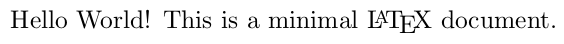
\includegraphics[scale=0.5,clip=true]{samples/example1.png}
%  \caption{Example \#1}
  \label{fig:example1}
\end{figure}

\end{frame}

%%%%%%%%%%%%%%%%%%%%%%%%%%%%%%%%%%%%%%%%%%%%%%%%%%%%%%%%%%%%%%%%%%%%%%%

\begin{frame}[fragile]
\frametitle{Document workflow}

\alert{Editor} (\texttt{`foobar.tex'}) $\to$ \alert{\LaTeX{} processor} (\texttt{`foobar.dvi'}) $\to$ \alert{display} (viewer/screen) $\to$ \alert{drivers} (\texttt{`foobar.ps'}, printer)

\definecolor{ivory2}{RGB}{238,238,224} % for background
% \definecolor{light-gray}{gray}{0.85}

\lstset{ 
emph={documentclass, begin, LaTeX},
emphstyle=\alert,
language=TeX,
frameround=fttt,
backgroundcolor=\color{ivory2},
keywordstyle=\color{red},
commentstyle=\color{gray},
basicstyle=\small,
stringstyle=\color{white},
}

\begin{lstlisting}[frame=trBL]
$ latex foobar.tex (`tex &latex foobar.tex')
$ dvips -o foobar.ps foobar.dvi (ps output)
$ pdflatex foobar.tex (pdf output)
$ hevea foobar.tex  (html output)
\end{lstlisting}

\end{frame}

%%%%%%%%%%%%%%%%%%%%%%%%%%%%%%%%%%%%%%%%%%%%%%%%%%%%%%%%%%%%%%%%%%%%%%%

\begin{frame}
\frametitle{DVI Output}

\begin{itemize}
\item Device independent file format (\texttt{.dvi}) 
\item Binary data independent on any specific image format, display hardware or printer.
\item A \alert{\LaTeX{} distribution} for processing (compiling) your \LaTeX{} source files into
PDF or DVI documents.
\item DVI is not a document encryption format.
\item Not support embedded fonts (fonts must be already installed).
\end{itemize}

\end{frame}

%%%%%%%%%%%%%%%%%%%%%%%%%%%%%%%%%%%%%%%%%%%%%%%%%%%%%%%%%%%%%%%%%%%%%%%

\begin{frame}
\frametitle{xdvi: DVI Previewer}

\begin{figure}
  \centering
	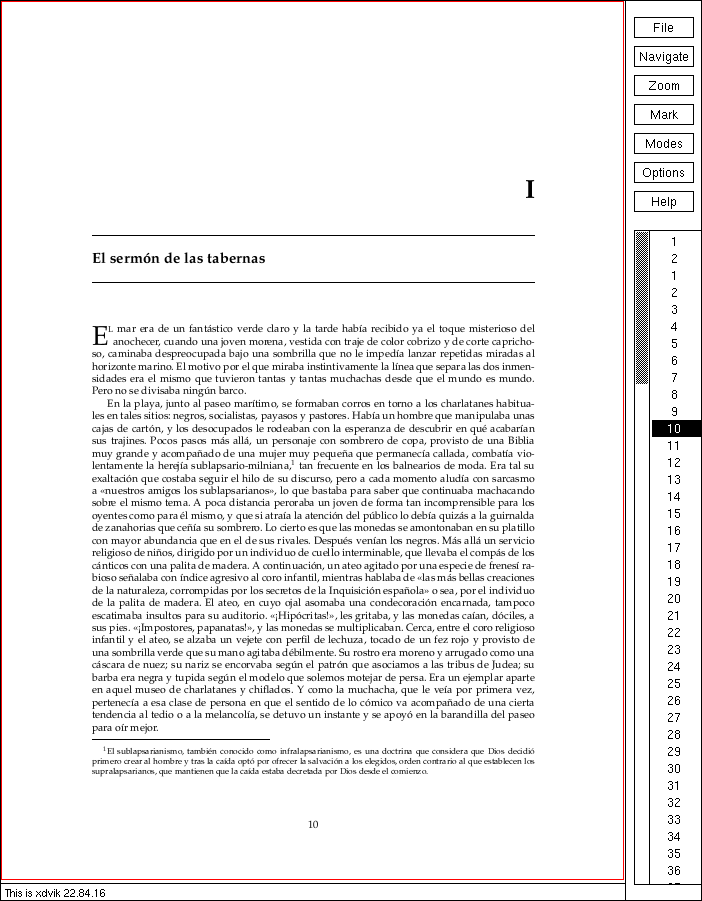
\includegraphics[scale=0.25,clip=true]{samples/xdvi.png}
%  \caption{Example \#1}
  \label{fig:xdvi}
\end{figure}

\end{frame}


%%%%%%%%%%%%%%%%%%%%%%%%%%%%%%%%%%%%%%%%%%%%%%%%%%%%%%%%%%%%%%%%%%%%%%%

\begin{frame}
\frametitle{\LaTeX{} Distributions}

There are pre-compiled \LaTeX{} distributions for different OS: 

\begin{itemize}
\item \alert{TeX Live} (Unix-like systems): Linux, BSD, Solaris, etc.
\item \alert{MacTeX} (TeX Live with the addition of Mac specific programs): \url{http://www.tug.org/mactex}
\item \alert{MiKTeX} (Windows): \url{http://www.miktex.org}
 
\end{itemize}

\end{frame}


%%%%%%%%%%%%%%%%%%%%%%%%%%%%%%%%%%%%%%%%%%%%%%%%%%%%%%%%%%%%%%%%%%%%%%%
\section{Basic Structures}
%%%%%%%%%%%%%%%%%%%%%%%%%%%%%%%%%%%%%%%%%%%%%%%%%%%%%%%%%%%%%%%%%%%%%%%

\subsection{Document Structure}


\begin{frame}
\frametitle{Document Structure}

Two main environments:

\begin{itemize}
\item \alert{Preamble:} commands and macros that affect the entire document.
\begin{itemize}
\item \alert{Top matter:} author, title, date, institution, etc. 
\end{itemize}
\item \alert{Document environment:} body text
\end{itemize}

\end{frame}

%%%%%%%%%%%%%%%%%%%%%%%%%%%%%%%%%%%%%%%%%%%%%%%%%%%%%%%%%%%%%%%%%%%%%%%

\begin{frame}[fragile]
\frametitle{Preamble}

\begin{itemize}
\item Everything from the start of the \LaTeX{} source file until the \texttt{\\begin\{document\}} command
\item It normally contains global commands that affect the entire document.
\end{itemize}

\definecolor{ivory2}{RGB}{238,238,224} % for background
% \definecolor{light-gray}{gray}{0.85}

\lstset{ 
emph={documentclass, begin, usepackage},
emphstyle=\alert,
language=TeX,
frameround=fttt,
backgroundcolor=\color{ivory2},
keywordstyle=\color{red},
commentstyle=\color{gray},
basicstyle=\small,
stringstyle=\color{white},
}

\begin{lstlisting}[frame=trBL]
\documentclass[options]{class}
\usepackage[options]{package} 
\end{lstlisting}

\small
\alert{class} (mandatory): book, article, report \\
\alert{package} (optional): to utilize external macros (\texttt{inputenc, amssymb}...)

\end{frame}

%%%%%%%%%%%%%%%%%%%%%%%%%%%%%%%%%%%%%%%%%%%%%%%%%%%%%%%%%%%%%%%%%%%%%%%

\begin{frame}[fragile]
\frametitle{Top Matter}

\normalsize

\begin{itemize}
\item Title, date
\item Information about the authors, such as name, address, email etc.
\end{itemize}

\definecolor{ivory2}{RGB}{238,238,224} % for background
% \definecolor{light-gray}{gray}{0.85}

\lstset{ 
% emph={documentclass, begin, title, author, date, maketitle, usepackage},
% emphstyle=\alert,
language=TeX,
frameround=fttt,
backgroundcolor=\color{ivory2},
% keywordstyle=\color{red},
commentstyle=\color{gray},
basicstyle=\small,
stringstyle=\color{white},
}

\begin{lstlisting}[frame=trBL]
\documentclass[11pt,a4paper,oneside]{report}
\usepackage[utf8]{inputenc} % utf-8 encoding
\usepackage{amssymb}  % math symbols

\begin{document}
\title{How to Structure a LaTeX Document}
\author{Andrew Roberts}
\date{December 2004}
\maketitle
\end{document}\end{lstlisting}


\end{frame}



%%%%%%%%%%%%%%%%%%%%%%%%%%%%%%%%%%%%%%%%%%%%%%%%%%%%%%%%%%%%%%%%%%%%%%%

\begin{frame}[fragile]
\frametitle{Body text}

\normalsize

\begin{itemize}
\item Abstract
\item Parts, chapters, sections, subsections, 
\item Appendices, Bibliography...
\end{itemize}

\definecolor{ivory2}{RGB}{238,238,224} % for background
% \definecolor{light-gray}{gray}{0.85}

\lstset{ 
emphstyle=\alert,
language=TeX,
frameround=fttt,
backgroundcolor=\color{ivory2},
keywordstyle=\color{red},
commentstyle=\color{gray},
stringstyle=\color{white},
}

\begin{lstlisting}[frame=trBL]
\begin{document}
  ... text mixed with local commands ...
\end{document}
\end{lstlisting}


\end{frame}



%%%%%%%%%%%%%%%%%%%%%%%%%%%%%%%%%%%%%%%%%%%%%%%%%%%%%%%%%%%%%%%%%%%%%%%


\begin{frame}[fragile] 
\frametitle{How to Structure a \LaTeX{} Document}

\LaTeX{} allows to structure documents with a variety of hierarchical constructs:

\definecolor{ivory2}{RGB}{238,238,224} % for background
% \definecolor{light-gray}{gray}{0.85}

\lstset{ 
emph={part, chapter, section, subsection, subsubsection},
emphstyle=\alert,
language=TeX,
frameround=fttt,
backgroundcolor=\color{ivory2},
keywordstyle=\color{red},
commentstyle=\color{gray},
% basicstyle=\small,
stringstyle=\color{white},
}

\begin{lstlisting}[frame=trBL]
\part{Part Title} 
\chapter{Chapter Title} %only books and reports
\section{Section Title} 	
\subsection{Subsection Title} 
\subsubsection{Subsubsection Title} 	
\end{lstlisting}


\end{frame}


%%%%%%%%%%%%%%%%%%%%%%%%%%%%%%%%%%%%%%%%%%%%%%%%%%%%%%%%%%%%%%%%%%%%%%%
\subsection{Fonts}

\begin{frame}[fragile]
\frametitle{Font Styles}


\definecolor{ivory2}{RGB}{238,238,224} % for background
% \definecolor{light-gray}{gray}{0.85}

\lstset{ 
emph={LaTeX, texttt, textsc, textit, textbf},
emphstyle=\alert,
language=TeX,
frameround=fttt,
backgroundcolor=\color{ivory2},
keywordstyle=\color{red},
commentstyle=\color{gray},
basicstyle=\small,
stringstyle=\color{white},
}

\begin{lstlisting}[frame=trBL]
\textit{...} % italics
\textbf{...} % bold
\texttt{...} % monospace - teletype
\textsc{...} % small capitals
\end{lstlisting}

Example: 

\begin{lstlisting}[frame=trBL, basicstyle=\footnotesize]
\LaTeX{} was \texttt{originally} written in 
\textbf{1984} by \textsc{Leslie Lamport} and has become 
the  \textit{dominant} method for using \TeX.
\end{lstlisting}

Output:
	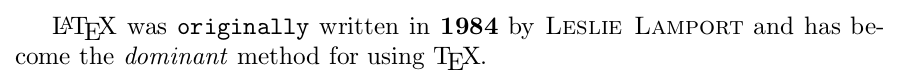
\includegraphics[scale=0.37,clip=true]{samples/example2.png}
\end{frame}

%%%%%%%%%%%%%%%%%%%%%%%%%%%%%%%%%%%%%%%%%%%%%%%%%%%%%%%%%%%%%%%%%%%%%%%


\begin{frame}[fragile]
\frametitle{Font Sizes}


\definecolor{ivory2}{RGB}{238,238,224} % for background
% \definecolor{light-gray}{gray}{0.85}

\lstset{ 
emph={documentclass, begin, LaTeX},
emphstyle=\alert,
language=TeX,
frameround=fttt,
backgroundcolor=\color{ivory2},
keywordstyle=\color{red},
commentstyle=\color{gray},
basicstyle=\small,
stringstyle=\color{white},
}

\begin{lstlisting}[frame=trBL]
\tiny  
\scriptsize 
\footnotesize 
\small 	      
\normalsize 
\large 	
\Large 	
\LARGE 	
\huge 	
\Huge 	
\end{lstlisting}

\small{Size related to font size default, declared in preamble (\texttt{documentclass})}

\end{frame}

%%%%%%%%%%%%%%%%%%%%%%%%%%%%%%%%%%%%%%%%%%%%%%%%%%%%%%%%%%%%%%%%%%%%%%%


\begin{frame}[fragile]
\frametitle{Font Sizes. Example}


\definecolor{ivory2}{RGB}{238,238,224} % for background
% \definecolor{light-gray}{gray}{0.85}

\lstset{ 
emph={tiny, normalsize, footnotesize, huge, LARGE},
emphstyle=\alert,
language=TeX,
frameround=fttt,
backgroundcolor=\color{ivory2},
% keywordstyle=\color{red},
commentstyle=\color{gray},
% basicstyle=\small,
stringstyle=\color{white},
}


\begin{lstlisting}[frame=trBL]
\LaTeX{} was \tiny originally written 
\normalsize  in \large 1984 \normalsize by 
\LARGE Leslie Lamport \normalsize and has 
become the \footnotesize dominant method 
\normalsize for using \huge \TeX.
\end{lstlisting}

\begin{block}{Output:}
\LaTeX{} was \tiny originally written \normalsize in 
\large 1984 \normalsize by \LARGE Leslie Lamport \normalsize 
and has become the \footnotesize dominant method \normalsize 
for using \huge \TeX.
\end{block}

\end{frame}


%%%%%%%%%%%%%%%%%%%%%%%%%%%%%%%%%%%%%%%%%%%%%%%%%%%%%%%%%%%%%%%%%%%%%%%



\begin{frame}
\frametitle{Some special features}

\begin{itemize}

\item Text aligned
\item $n > 1$ blank lines and empty spaces: one line or one space
\item Start a new paragraph: \textbackslash\textbackslash
\item Hyphenate the word (exceptional cases): \texttt{man\textbackslash-u\textbackslash-script}
\item \texttt{\textbackslash newline}, \texttt{\textbackslash newpage}

\end{itemize}

\end{frame}



%%%%%%%%%%%%%%%%%%%%%%%%%%%%%%%%%%%%%%%%%%%%%%%%%%%%%%%%%%%%%%%%%%%%%%%

\subsection{Environments}

\begin{frame}[fragile]
\frametitle{Environments}


\definecolor{ivory2}{RGB}{238,238,224} % for background
% \definecolor{light-gray}{gray}{0.85}

\lstset{ 
emph={begin},
emphstyle=\alert,
language=TeX,
frameround=fttt,
backgroundcolor=\color{ivory2},
keywordstyle=\color{red},
commentstyle=\color{gray},
basicstyle=\small,
stringstyle=\color{white},
}

\begin{lstlisting}[frame=trBL]
\begin{environment name}
\end{environment name} 
\end{lstlisting}

Environments: \texttt{center, itemize, enumerate, figure, flushright, quotation...}

\end{frame}


%%%%%%%%%%%%%%%%%%%%%%%%%%%%%%%%%%%%%%%%%%%%%%%%%%%%%%%%%%%%%%%%%%%%%%%

\begin{frame}[fragile]
\frametitle{Environments: example}

\normalsize

\definecolor{ivory2}{RGB}{238,238,224} % for background
% \definecolor{light-gray}{gray}{0.85}

\lstset{ 
emph={begin},
emphstyle=\alert,
language=TeX,
frameround=fttt,
backgroundcolor=\color{ivory2},
keywordstyle=\color{red},
commentstyle=\color{gray},
basicstyle=\small,
stringstyle=\color{white},
}

\begin{lstlisting}[frame=trBL]
Some FOSS Licenses:
\begin{enumerate}
\item BSD license
\item GPL license
\item CDDL license
\end{enumerate}\end{lstlisting}

Output: \\
\medskip
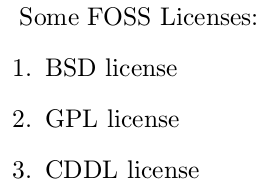
\includegraphics[scale=0.35,clip=true]{samples/example3.png}

\end{frame}


\subsection{A complete document}
%%%%%%%%%%%%%%%%%%%%%%%%%%%%%%%%%%%%%%%%%%%%%%%%%%%%%%%%%%%%%%%%%%%%%%%

\begin{frame}[fragile] 
\frametitle{A complete document}

\definecolor{ivory2}{RGB}{238,238,224} % for background
% \definecolor{light-gray}{gray}{0.85}

\lstset{ 
emph={documentclass, begin, LaTeX},
emphstyle=\alert,
language=TeX,
frameround=fttt,
backgroundcolor=\color{ivory2},
keywordstyle=\color{red},
commentstyle=\color{gray},
basicstyle=\footnotesize,
stringstyle=\color{white},
}

\begin{lstlisting}[frame=trBL]
\usepackage[utf8]{inputenc}
\title{The beauty of \TeX}
\author{Donald E. Knuth}
\date{\1979}

\begin{document}
  \maketitle

% This is the comment body.
``Mathematical books and journals do not look as 
beautiful as they used to. It is not that their 
mathematical content is unsatisfactory, rather that the 
old and well-developed traditions of typesetting have 
become too expensive. Fortunately, it now appears that 
mathematics itself can be used to solve this problem.''

\end{document}

\end{lstlisting} 
% \end{boxedverbatim} 

\end{frame}

%%%%%%%%%%%%%%%%%%%%%%%%%%%%%%%%%%%%%%%%%%%%%%%%%%%%%%%%%%%%%%%%%%%%%%%

\begin{frame}[fragile] 
\frametitle{A complete document}

\begin{figure}
  \centering
	
\includegraphics[scale=0.35,clip=true]{samples/example4.png}
%  \caption{Example \#1}
  \label{fig:example1}
\end{figure}

\end{frame}


%%%%%%%%%%%%%%%%%%%%%%%%%%%%%%%%%%%%%%%%%%%%%%%%%%%%%%%%%%%%%%%%%%%%%%%
\section{References}
%%%%%%%%%%%%%%%%%%%%%%%%%%%%%%%%%%%%%%%%%%%%%%%%%%%%%%%%%%%%%%%%%%%%%%%

\begin{frame} 
\frametitle{References}

\begin{itemize}
\item \textsc{Lamport}, Leslie. \textit{\LaTeX: A document preparation system}, Addison-Wesley, Reading, Massachusetts, second edition, 1994.
\item \textsc{Knuth}, Donald E. \textit{The \TeX book, Volume A of Computers and Typesetting}, Addison-Wesley, Reading, Massachusetts, second edition, 1984.
\item CTAN: the authoritative collection of materials related to the TeX typesetting system. \url{http://www.ctan.org}
\item Guide to the \LaTeX markup language: \url{http://en.wikibooks.org/wiki/LaTeX}
\end{itemize}

\end{frame}

%%%%%%%%%%%%%%%%%%%%%%%%%%%%%%%%%%%%%%%%%%%%%%%%%%%%%%%%%%%%%%%%%%%%%%%

\begin{frame} 
\frametitle{References (Spanish)}

\begin{itemize}
\item \textsc{Sanguino-Botella}, Javier. \textit{Iniciación a \LaTeX2e: Un sistema para preparar documentos}, Addison-Wesley, 1997.
\item \textsc{VV.AA.} \textit{\LaTeX: Una imprenta en sus manos}, ADI, 2000.
\item \TeX{} y tipografía (web de Javier Bezos): \url{http://www.tex-tipografia.com}
\item CervanTeX: Grupo de usuarios hispanohablantes de \TeX: \url{http://www.cervantex.es/}
\end{itemize}

\end{frame}


%%%%%%%%%%%%%%%%%%%%%%%%%%%%%%%%%%%%%%%%%%%%%%%%%%%%%%%%%%%%%%%%%%%%%%%

% Final slide
\usebackgroundtemplate{
\includegraphics[width=\paperwidth]{format/libresoft-bg}}

\frame{
\maketitle
\begin{center}

\includegraphics[width=6cm]{format/gsyc-urjc}
\end{center}
}

\end{document}

Ejemplos tipografía vs word:
http://nitens.org/taraborelli/latex
